\chapter{\IfLanguageName{dutch}{Stand van zaken}{State of the art}}
\label{ch:stand-van-zaken}

% Tip: Begin elk hoofdstuk met een paragraaf inleiding die beschrijft hoe
% dit hoofdstuk past binnen het geheel van de bachelorproef. Geef in het
% bijzonder aan wat de link is met het vorige en volgende hoofdstuk.

% : Pas na deze inleidende paragraaf komt de eerste sectiehoofding.

``Kan \textit{elderspeak} gedetecteerd worden door Artificiële Intelligentie en kan dit toegepast worden in de praktijk?'', is de centrale onderzoeksvraag.
Om te kunnen staven of dit wel degelijk mogelijk is, moeten twee begrippen uitgelegd en begrepen worden.
Er zal dus eerst beschreven worden wat \textit{elderspeak} precies is, hoe het ontstaat, wat de schadelijke effecten zijn, maar ook wat de eigenschappen zijn en hoe kan met het voorkomen?
Ten tweede moeten we ook begrijpen wat Artificiële Intelligentie is, daarbij alle verschillende types, vormen en gradaties ervan.

\section{Elderspeak}

\subsection{Definitie van elderspeak}

Het begrip \textit{elderspeak}, ook \textit{secondary babytalk} genoemd, kent verschillende definities. \textcite{Kemper1998} omschrijft het begrip als volgt:
``Elderspeak is a simplified speech register with exaggerated pitch and intonation, simplified grammar, limited vocabulary and slow rate of delivery.''

Daarnaast beschrijft \textcite{Williams2011} het begrip als volgt:
``Elderspeak is a common intergenerational speech style used by younger persons in communication with older adults in a variety of community and health care settings. Based on negative stereotypes of older adults as less competent communicators, younger speakers (in this case nursing home staff) modify their communication with nursing home residents by simplifying the vocabulary and grammar and by adding clarifications such as repetitions and altered prosody.'' Het omvat dus de stereotiepe communicatie tussen ouderen en jongeren.

\subsection{Ontstaan van elderspeak}
Er zijn verschillende communicatietheorieën die het ontstaan van \textit{elderspeak} kunnen verklaren.

De Communicatie Accommodatie Theorie (CAT) beschrijft hoe mensen hun gespreksstijl aan hun gesprekspartner aanpassen en stelt dat deze aanpassingen een manier zijn om waarden en attitudes te uiten, aldus \textcite{Campens2021}. Dat verschil in communiceren word convergeren genoemd. Dit is wanneer een gesprekspartner in de communicatie tracht af te stemmen op de communicatiestijl van de andere, waardoor twee gesprekspartners op de zelfde golflengte komen te zitten. Dit brengt mee dat de gesprekspartner beter luistert naar de spreker en de spreker voor de gesprekspartner voorspelbaarder wordt.

Bij \textit{elderspeak} convergeert die stijl echter in een extreme vorm. De gesprekspartner laat zich te veel leiden door het stereotiepe beeld van ouderen. Het CAT-model stelt dat de jongere zich in zo'n geval niet aanpast aan de oudere gesprekspartner, maar wel aan dat stereotiepe beeld. Hierdoor zal \textit{elderspeak} versterkt worden tijdens een gesprek~\autocite{Hehman2015}.

De tweede communicatietheorie, namelijk het Communication Predicament of Ageing Model (CPA), beschrijft dat het stereotiepe beeld gestimuleerd kan worden. Dit wordt aangemoedigd door de omgeving, zoals een woon-zorgcentrum, en kenmerken, zoals een hoorapparaat of wandelstok~\autocite{Hehman2015}.

In tegenstelling tot de twee vorige communicatiemodellen, probeert het Communicatie Enhancement of Ageing model (CEA) de vicieuze cirkel van het CPA-model te doorbreken. \textcite{Campens2021} beschrijft dit als volgt: ``Het model stelt voor om de gespreksstijl op de individuele (oudere) gesprekspartner af te stemmen en een person-centered-approach te hanteren, eerder dan een category-based-approach (zoals bij het CPA-model het geval is).''. Dit kan bekomen worden door systematische beoordeling van de individuele kenmerken van de gesprekspartner bij het begin van een conversatie. Wanneer er aanpassingen nodig zijn, moet er opnieuw een beoordeling plaatsvinden. Het model stelt dat er op die manier positieve resultaten kunnen bekomen worden voor beide gesprekspartners zoals empowerment, toegenomen competenties, tevredenheid, effectieve communicatie etc.\~\autocite{Hehman2015}.

\subsection{Gevolgen van elderspeak}
Zorgpersoneel probeert ouderen op hun gemak te stellen, vriendelijk over te komen, de boodschap van een gesprek op een duidelijke en effectieve wijze over te brengen en een betere samenwerking te verkrijgen. Hierdoor past men (on)bewust \textit{elderspeak} toe, maar met de beste bedoelingen~\autocite{Grimme2015}.

Door \textit{elderspeak} toe te passen komen er negatieve gevolgen tevoorschijn bij ouderen. Zo krijgen ze het gevoel dat ze hulpeloos en afhankelijk zijn. Het bedreigt hun zelfbeeld, zelfrespect en het welzijn. Bovendien kan het depressieve gevoelens opwekken die zowel fysieke als cognitieve achteruitgang in de hand kunnen werken. Hierdoor zullen sommige ouderen sociale interactie vermijden en mogelijk sociaal geïsoleerd geraken~\autocite{Williams2011a}.

Het is dus belangrijk dat elderspeak vermeden wordt, want het ervaren van sociale betrokkenheid gaat gepaard met een toename van de tevredenheid over het leven~\autocite{Williams2011a}.

\subsection{Kenmerken van elderspeak}
De kenmerken komen overeen met de communicatiestijl die men hanteert wanneer men tegen (afhankelijke) kinderen praat. Vandaar dat \textit{elderspeak} ook wel als \textit{secondary baby talk} wordt benoemd. \textcite{Campens2021} somt de kenmerken als volgt op:

\begin{itemize}
    \item Langzaam spreken
    \item Verhoogde toonhoogte
    \item Verhoogd stemvolume
    \item Overdreven intonatie
    \item Vereenvoudigd woordgebruik, gebruik van verkleinwoorden en/of ongepaste bijnamen of troetelnamen
    \item Verminderde grammaticale complexiteit (bv.\ voornamelijk enkelvoudige zinnen)
    \item Gebruik van collectieve voornaamwoorden (bijvoorbeeld ``we'' in plaats van ``jij'')
    \item Veelvuldig gebruik van (bevestigende) tussenwerpsels (zoals ``hé'' of ``voilà'')
    \item Gewijzigd non-verbaal gedrag (bv.\ langdurig oogcontact, extra gebaren, te dichtbij komen)
    \item Veelvuldige verduidelijking en herhaling
\end{itemize}

Ten slotte is het belangrijk om te beseffen dat bij \textit{elderspeak} de inhoud van de boodschap, die de zorgverlener wil overbrengen, niet wijzigt. Wel verandert de wijze waarop de boodschap wordt overgebracht door het gebruik van een infantiliserende communicatiestijl, aldus \textcite{Campens2021}.

\subsection{Tips om elderspeak te voorkomen?}

De onderstaande tips zijn er enkelen die \textcite{Wick2007} meegeven om \textit{elderspeak} te voorkomen:

\begin{itemize}
    \item Spreek personen aan met de naam waarmee ze willen aangesproken worden. Gebruik geen collectieve voornaamwoorden als die niet van toepassing zijn.
    \item Als een persoon een zorgverlener toelaat om hem of haar met zijn voornaam aan te spreken, ga er dan niet van uit dat deze “toestemming” voor alle zorgverleners geldt. De mate van intimiteit varieert, waardoor elke zorgverlener moet nagaan hoe hij of zij zijn of haar gesprekspartner mag aanspreken.
    \item Vermijd het gebruik van troetelnamen en overmatige intieme liefkozingen, tenzij de gesprekspartner uitdrukkelijk aangeeft dat hij of zij zo wil aangesproken worden.
    \item Wees je bewust van je non-verbaal gedrag.
    \item Verhoog je stemvolume (in beperkte mate) enkel en alleen wanneer de gesprekspartner hardhorig is. Verhoging van je stemvolume betekent geen verhoging van je stemhoogte. Wees je ervan bewust dat niet elke oudere gesprekspartner hardhorig is.
    \item Herhaling en verminderde grammaticale complexiteit hebben een plaats als de gesprekspartner je niet begrepen heeft.
    \item Vermijd korte, langzaam en met overdreven intonatie uitgesproken zinnen.
    \item Vermijd het gebruik van verkleinwoorden, aangezien die het gevoel van afhankelijkheid kunnen versterken en denigrerend kunnen geïnterpreteerd worden.
    \item Vermijd overdreven directieve boodschappen en bied keuzevrijheid.
    \item Hanteer een beleefd taalgebruik en beleefde omgangsvormen (bv.\ op de kamerdeur kloppen alvorens de kamer binnen te gaan).
\end{itemize}

\clearpage

\section{Artificiële Intelligentie}
\subsection{Definitie van AI?}
Er zijn bijzonder veel beschrijvingen van AI, maar een combinatie van bronnen geeft het meest accurate beeld.

Volgens \textcite{Oracle2014} heeft AI (kunstmatige intelligentie) betrekking op systemen of machines die onze eigen intelligentie nabootsen om taken uit te voeren en die zichzelf tijdens dat proces kunnen verbeteren op basis van de vergaarde informatie.

Het \textcite{EuropeesParlement2020} geeft de volgende definitie aan artificiële intelligentie (of kunstmatige intelligentie): ``AI is de mogelijkheid van een machine om mensachtige vaardigheden te vertonen - zoals redeneren, leren, plannen en creativiteit.
AI maakt het voor technische systemen mogelijk om hun omgeving waar te nemen, om om te gaan met deze waarnemingen en problemen op te lossen om een specifiek doel te bereiken. De computer ontvangt data - reeds voorbereid en verzameld via eigen sensoren, zoals een camera - verwerkt deze en reageert erop.
AI-systemen zijn in staat om hun gedrag in zekere mate aan te passen door het effect van vorige acties te analyseren en autonoom te werken.''

Samengevat is AI een technisch systeem dat opereert via complexe/grootschalige informatievergaring, maar waarbij het systeem vooral ook zichzelf aanpast op basis van die vergaarde informatie en op die manier menselijke intelligentie nabootst.

\subsection{Vormen van AI}
Artificiële Intelligentie is een verzamelnaam voor twee soorten algoritmes. Zo is er enerzijds \textit{machine learning} en anderzijds \textit{deep learning}~\autocite{Kavlakoglu2020}.
Dit kan mooi geïllustreerd worden a.d.h.v.\ figuur~\ref{fig:soorten_ai_diagram}.

\begin{figure}
    \centering
    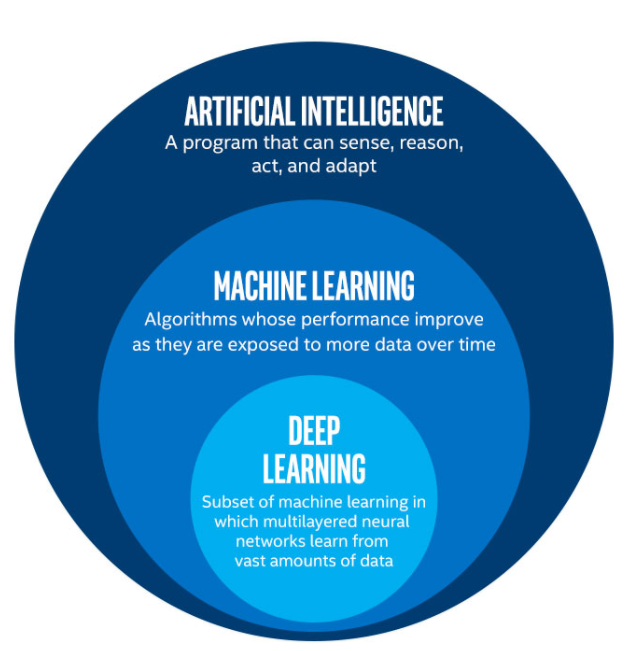
\includegraphics[width=0.6\textwidth]{./img/ai_fields}
    \caption{\label{fig:soorten_ai_diagram} Soorten AI in diagram~\autocite{Bansal2019}}
\end{figure}

\subsection{Machine learning}
\textit{Machine learning} of machinaal leren is het deelgebied van kunstmatige intelligentie dat computers het vermogen geeft te leren zonder expliciet geprogrammeerd te zijn, aldus \textcite{Lievens2021}. Machinaal leren heeft drie type, namelijk \textit{supervised learning} of gesuperviseerd leren, \textit{unsupervised learning} of leren zonder toezicht en \textit{reinforcement learning} of leren door bekrachtiging.

\subsubsection{Supervised learning}
Een definitie over \textit{supervised learning}, gegeven door \textcite{Lievens2021}, gaat als volgt: ``De taak van \textit{supervised learning} is een hypothese op te bouwen op basis van een reeks gelabelde trainingsgegevens. Deze hypothese kan dan worden gebruikt om het label voor een (nieuwe) input te voorspellen. Wanneer het label een reëel getal is, spreekt men van een regressieprobleem; wanneer het label beperkt is tot een (beperkt) aantal vooraf gedefinieerde klassen, wordt het probleem een classificatieprobleem genoemd.''
De visuele voorstelling van beide problemen is te vinden in figuur~\ref{fig:classification_vs_regression}.

Een voorbeeld van het regressieprobleem is het voorspellen van huisprijzen. De input van het model is dan een reeks vectoren die de eigenschappen van het huis voorstellen zoals aantal slaapkamers, oppervlakte, bouwjaar etc.

Voorbeelden van het classificatieprobleem zijn spamdetectie, nummerherkenning of diabetesdetectie. Elk hebben ze een beperkt aantal outputklassen. Bij spamdetectie zijn er twee vooraf gedefinieerde klassen: spam en geen spam. Bij nummerherkenning zijn er 10 klassen (0 t.e.m.\ 9) en bij diabetesdetectie kunnen er drie klassen aanwezig zijn (geen diabetes, pre-diabetes en diabetes).

\begin{figure}
    \centering
    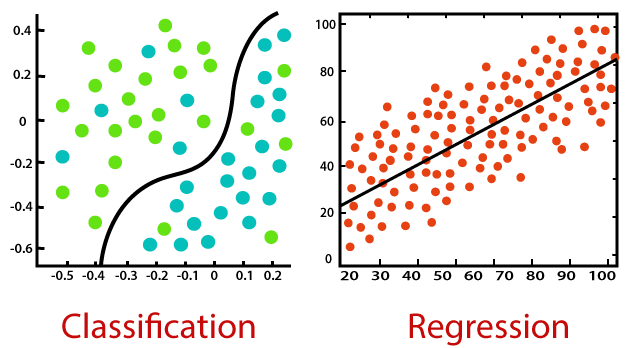
\includegraphics[width=0.75\textwidth]{./img/classification_regression}
    \caption{\label{fig:classification_vs_regression} Classification vs.\ Regression~\autocite{JavaTpoint2021}.}
\end{figure}

\subsubsection{Unsupervised learning}
\textcite{Lievens2021} omschrijft \textit{unsupervised learning} als de taak van het ontdekken van structuur in een ongelabelde gegevensreeks.

De meest prominente taak bij \textit{unsupervised learning} is \textit{clustering}, d.w.z.\ de ontdekking van coherente groepen. Andere mogelijke taken zijn anomaliedetectie en hoofdcomponentenanalyse (PCA).

Een voorbeeld van clustering is marktsegmentatie waarbij klanten worden opgedeeld in verschillende segmenten zoals trouwe klant, mogelijke vertrekkende klant, ontevreden klant etc. Op basis van aankoopdata, tijdstippen en online activiteit kan men de klanten indelen in clusters. Die informatie kan dan weer gebruikt worden om mensen die behoren tot bepaalde clusters korting te geven of te contacteren i.v.m.\ hun ontevredenheid.
Daarnaast zijn er algoritmen die fraude opsporen door het analyseren van abnormaal gedrag op een website. Dit is dan een voorbeeld van anomaliedetectie.
Bij PCA wordt de data gereduceerd zodat de minder relevante data weggefilterd wordt uit de dataset.

\subsubsection{Reinforcement learning}
\textcite{Lievens2021} beschrijft \textit{reinforcement learning} als een techniek die niet echt een dataset gebruikt, maar wel een identiteit die leeft in een (on)bekende wereld. Die identiteit krijgt dan beloningssignalen. De opdracht is dan om uit te zoeken welke regels leiden tot een grote beloning.

Het bekendste voorbeeld van \textit{reinforcement learning} is dat van zelfrijdende wagens. Hierbij moet het model zelf aanleren in welke mate het moet remmen, gas geven en sturen. Dit is een lang en iteratief proces waarbij het model zichzelf de hele tijd bijstuurt en leert van wat het net ervaren heeft.

\subsection{Deep Learning}
\textit{Deep learning} is het onderdeel van \textit{machine learning} dat neurale netwerken bevat.
``Een artificieel neuraal netwerk bestaat uit een groot aantal eenvoudige rekenende eenheden, units of neuronen die de volgende eigenschap hebben: `Als de (gewogen) input van een neuron groot is, zal het 'vuren' en dit neuron zal een grote waarde op zijn axon zetten. Bovendien zijn deze eenheden verbonden door middel van gerichte links waarbij een reëel getal de sterkte van elke verbinding aangeeft.'', aldus \textcite{Lievens2021} in zijn cursus \textit{Distributed Databases}.

De systematische voorstelling van een neuron is te vinden in figuur~\ref{fig:neuron}.
Een volledig neuraal netwerk zoals in figuur~\ref{fig:layers}. De data wordt gevoed aan de \textit{input layer}. Daarna komen een x-aantal \textit{hidden layers} die dan de bewerkingen uitvoeren en als laatste stap heb je de \textit{output layer}. Het aantal \textit{nodes} of knopen in de \textit{output layer} is gelijk aan het aantal klassen dat een probleem heeft. Als er een \textit{deep learning}-model gemaakt wordt van het detecteren van spam, dan zou de \textit{output layer} twee knopen moeten hebben.

\begin{figure}
    \centering
    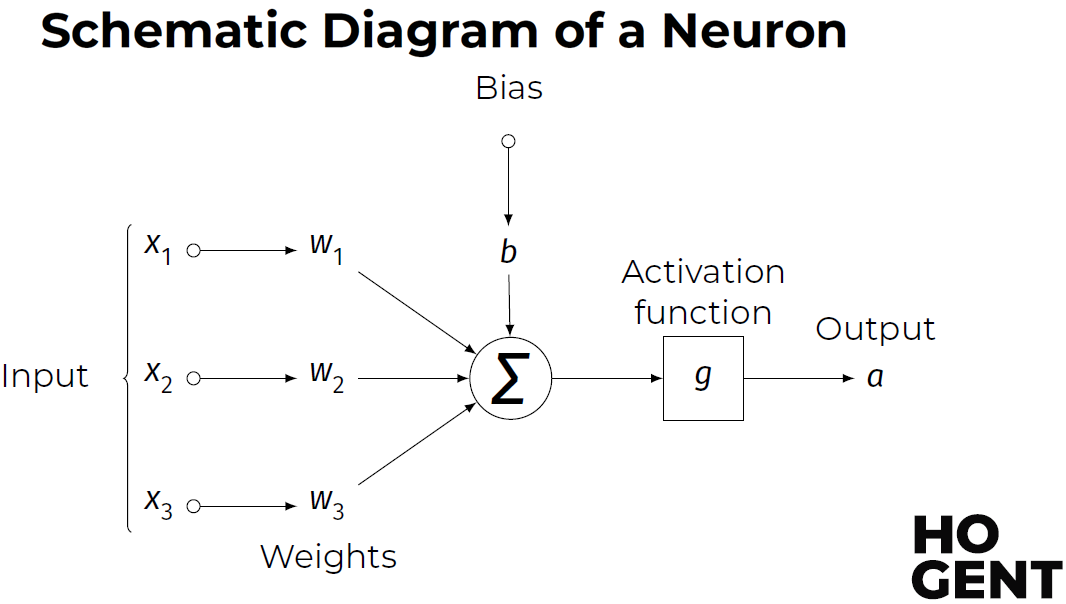
\includegraphics[width=1\textwidth]{./img/neuron}
    \caption{\label{fig:neuron} Systematische voorstelling van een Neuron~\autocite{Lievens2021}.}
\end{figure}

\begin{figure}
    \centering
    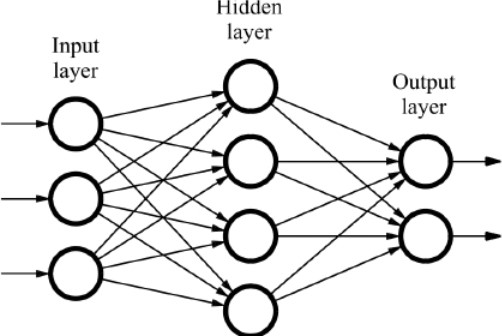
\includegraphics[width=.5\textwidth]{./img/layers}
    \caption{\label{fig:layers} Layers van een artificieel neuraal netwerk~\autocite{Lievens2021}.}
\end{figure}


\section{AI-technieken die gebruikt worden om elderspeak te detecteren}

\subsection{NLP of natural language processing}
Om te kunnen detecteren of de spreker verkleinwoorden, troetelnamen, collectieve voornaamwoorden of te veel tussenwerpsels gebruikt, moet het model, of eerder gezegd de Python-bibliotheek die het model bevat, weten of deze eigenschappen voorkomen. Hiervoor moeten we gebruik maken van \textit{natural language processing}-bibliotheken of afgekort NLP.

\textit{Natural language processing} of ``natuurlijke taalverwerking'' situeert zich in de tak van de kunstmatige intelligentie. NLP behoort deels tot \textit{machine learning} en deels tot \textit{deep learning} \autocite{Kleinings2022}. De visuele voorstelling van die verhoudingen is te vinden in figuur~\ref{fig:nlp_field}.

Volgens \textcite{Kleinings2022} is die natuurlijke taalverwerking een technologie die gebruikt wordt om computers te helpen om natuurlijke menselijke taal te begrijpen en te interpreteren.

NLP combineert computationele linguïstiek (op regels gebaseerde modellering van menselijke taal) met statistische, \textit{machine learning}- en \textit{deep learning}-modellen. Samen stellen deze technologieën computers in staat menselijke taal in de vorm van tekst of spraakgegevens te verwerken en de volledige betekenis ervan te ``begrijpen'', met inbegrip van bedoeling en het sentiment van de spreker of schrijver.~\autocite{IBMCloudEducation2021}

NLP stuurt computerprogramma's aan die tekst van de ene taal naar de andere kunnen vertalen, die reageren op gesproken opdrachten en die grote hoeveelheden tekst samenvatten, zelfs in realtime. Enkele voorbeelden van NLP-systemen in het dagelijkse leven zijn: spraakgestuurde GPS-systemen, digitale assistenten, spraak-naar-tekst dicteersoftware (o.a.\ in smartphones of Microsoft Word), chatbots voor de klantenservice en andere `gemakken' voor de consument. Maar NLP speelt ook een steeds grotere rol in bedrijfsoplossingen die helpen bij het stroomlijnen van de bedrijfsvoering, het verhogen van de productiviteit van werknemers en het vereenvoudigen van bedrijfskritische bedrijfsprocessen, aldus \textcite{IBMCloudEducation2021}.

\begin{figure}
    \centering
    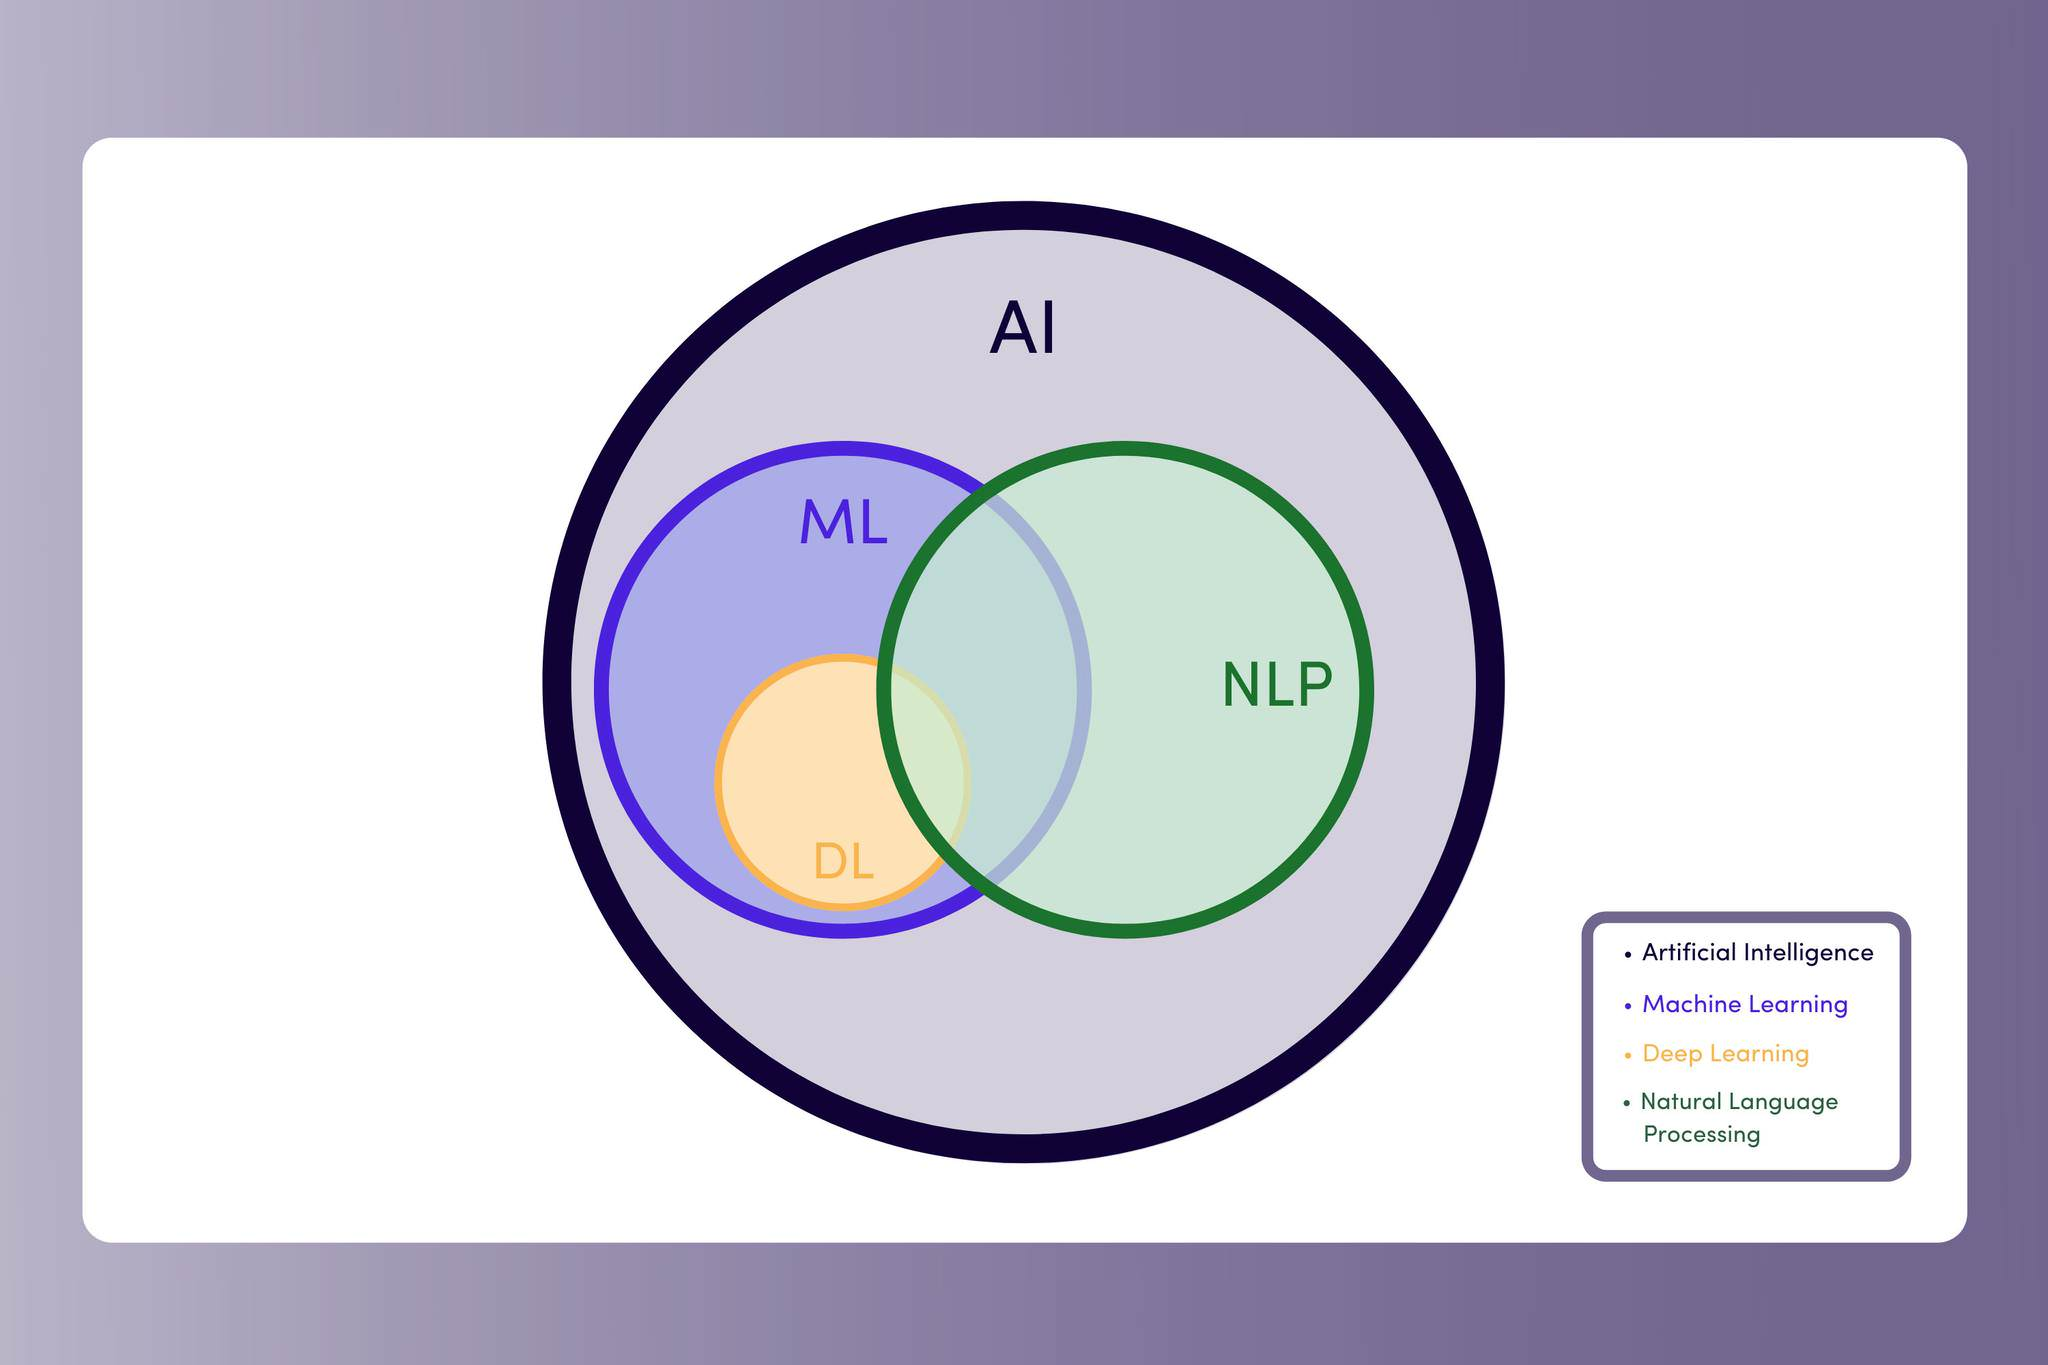
\includegraphics[width=.8\textwidth]{./img/nlp_field_ai.jpeg}
    \caption{\label{fig:nlp_field} Situering van NLP binnen het AI-veld~\autocite{Kleinings2022}.}
\end{figure}

\subsubsection{Waarom is het analyseren van taal moeilijk?}
Volgens \textcite{Kleinings2022} zijn er vele redenen waarom het verwerken van taal door een computer of AI-systeem nog steeds moeilijk is en zal blijven.

Eerst en vooral heb je alle linguïstische regels per taal. Zo zijn er meer dan 6500 talen die gesproken worden en die elke hun eigen regels hebben.
Daarnaast is er het probleem van de uniformiteit. Om taal te kunnen verwerken moet die eerst omgezet worden in een systeem of formaat dat de computer kan begrijpen. Door middel van machinaal leren identificeert het model ongestructureerde taal, en zet deze om naar bruikbare, niet-dubbelzinnige informatie. De computer kan dit begrijpen en er verder mee rekenen. Dit onderdeel wordt de \textit{pre-processing} genoemd.

Bovendien speelt de context NLP ook vaak parten. \textit{Natural Language Processing} werkt immers fundamenteel door de hiërarchie van linguïstische dictie tussen elk woord te begrijpen en deze om te zetten in een vorm die computers kunnen interpreteren. Onze talen zijn niet eenvoudig, zo hebben woorden meerdere betekenissen die alleen begrepen worden door het verschil in context.~\autocite{Kleinings2022} Een voorbeeld hiervan is het woord ``bank''. In de ene context is het de financiële instelling en in een andere context is het de rustbank in het park.

Als laatste kan de toon van de stem ook nog verschillen. Mensen kunnen d.m.v.\ intonatie en toonhoogte sarcasme of ironie uiten, zodat de zin een andere betekenis krijgt. Het kost veel moeite om om dit correct te interpreteren.

\subsubsection{Werking van NLP}
NLP is niet één statische methode, maar een ketting van manipulaties van de tekst zodat er meer lagen informatie tevoorschijn komen. Dit wordt gerealiseerd met neurale netwerken waarbij elke node een bepaalde functie uitvoert.
Er zijn vier grote stappen i.v.m.\ de taalverwerking namelijk morfologie, syntaxis, semantiek en pragmatiek, schrijft \textcite{Kleinings2022}. Dit is te lezen is op een \textit{low-code/no-code} platform, genaamd Levity, dat dus veel kennis heeft over AI. Daar kan men blokken slepen en gebruiken om een AI-model op te stellen.

Met behulp van morfologie kan er per woord een type geclassificeerd worden zoals een zelfstandig naamwoord, bijvoeglijk naamwoord, voornaamwoord, lidwoord enzovoort. Denk hierbij aan het voorbeeld met de bank.

Om de syntaxis aan te leren zijn er twee manieren. Enerzijds kunnen er woorden gelabeld worden waarbij er aangeduid wordt dat woord A de stam is, woord B de 2\textsuperscript{e} persoon enkelvoud, woord C het voltooid deelwoord etc. Anderzijds kan er een \textit{unsupervised machine learning} model gemaakt worden waarbij de computer de regels afleidt uit verschillende gelabelde teksten, en die logica gebruikt om nieuwe, niet-gelabelde, teksten te begrijpen.

Daarnaast is het ook aan te raden dat stopwoorden verwijderd worden als het model de tekst wil begrijpen. Stopwoorden zoals ``een, de, euh, inderdaad, echt, oké, eigenlijk, allez, etc.'' moeten verwijderd worden. Daarbij aansluitend zijn er twee andere methoden. Enerzijds lemmatiseren, waarbij  werkwoorden naar de tegenwoordige tijd veranderd worden.
Anderzijds is er stamming, waarbij er prefixen of affixen verwijderd worden. Een voorbeeld van conversie is dan: ``wij dachten'' naar ``denk''. Woorden worden daarnaast ook vervangen door meer gebruikte synoniemen zoals van ``enorm'' naar ``groot''.

Als laatste systeem of layer bestaat er \textit{tokenization}. Dit is het proces waarbij het systeem de zin indeelt in verschillende eenheden waaruit informatie kan gehaald worden.
Er kan een \textit{token} gekozen worden op basis van regels, leestekens, spaties, maar dit geeft wel steeds een ander resultaat, wat geïllustreerd is in figuur~\ref{fig:tokens}. Hoe die \textit{tokenization} zich verhoudt met die \textit{layer} van het \textit{deep learning}-NLP-model is te vinden in figuur~\ref{fig:tokens_verhouding_dl}.

\begin{figure}
    \centering
    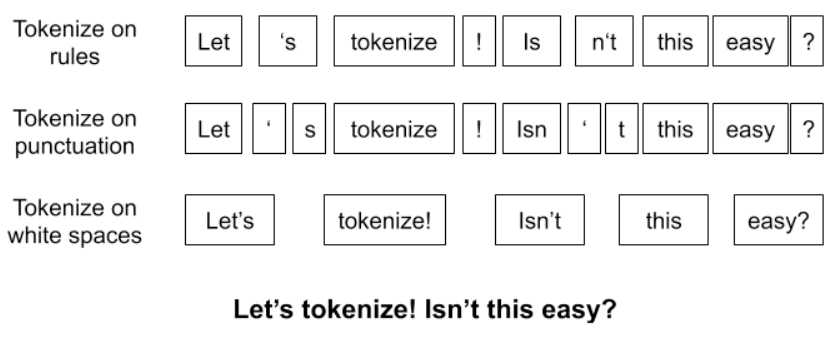
\includegraphics[width=1\textwidth]{./img/tokenize_manier}
    \caption{\label{fig:tokens} Manieren om een zin om te delen volgens een \textit{token}~\autocite{Horan2020}.}
\end{figure}

\begin{figure}
    \centering
    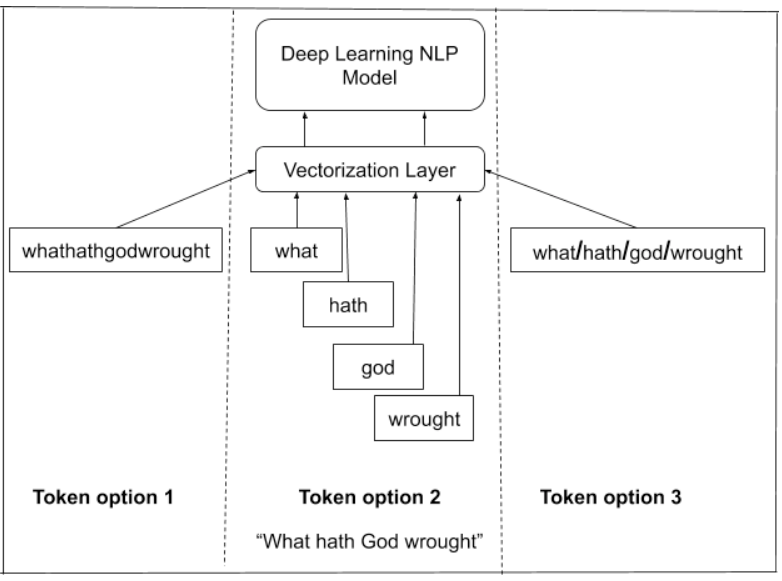
\includegraphics[width=0.8\textwidth]{./img/tokenization-1}
    \caption{\label{fig:tokens_verhouding_dl}Verhouding \textit{deep learning}-NLP-model met de layers en de verschillende \textit{tokens}~\autocite{Horan2020}.}
\end{figure}

%\clearpage

\subsection{Filteren van achtergrondlawaai}
Volgens \textcite{Jung2021} helpen \textit{convolutional neural networks} of CNN's bijzonder veel om achtergrondlawaai weg te filteren. Een CNN is een specifieke opstelling van een \textit{deep learning}-model waarbij een data-array van twee of meer dimensies, zoals een afbeelding of geluidsfragment, wordt gestapeld door een veelvoud van tweedimensionale filters.

Om achtergrondlawaai weg te werken zijn AI-gebaseerde filters, zoals de \textit{short-time Fourier transform} of STFT, ideaal. De STFT-filter verbetert in het algemeen de kwaliteit van het inkomende geluidssignaal door ruis uit het geluidssignaal te verwijderen.
De STFT is een Fourier-gerelateerde transformatie die wordt gebruikt om de sinusoïdale frequentie- en fase-inhoud van plaatselijke delen van een signaal te bepalen terwijl dit in de tijd verandert, zie figuur~\ref{fig:conversion}. In de praktijk worden STFT's berekend door een geluidssignaal op te delen in kortere segmenten van gelijke lengte en de Fouriertransformatie afzonderlijk te berekenen voor elk korter segment. Aldus wordt het Fourier-spectrum voor elk korter segment onthuld. Gewoonlijk zet men dan de veranderende spectra uit in functie van de tijd; de grafiek staat bekend als een spectrogram of watervalgrafiek, zie figuur~\ref{fig:The_original_noise-removed_audio}.~\autocite{Jung2021}

\begin{figure}
    \centering
    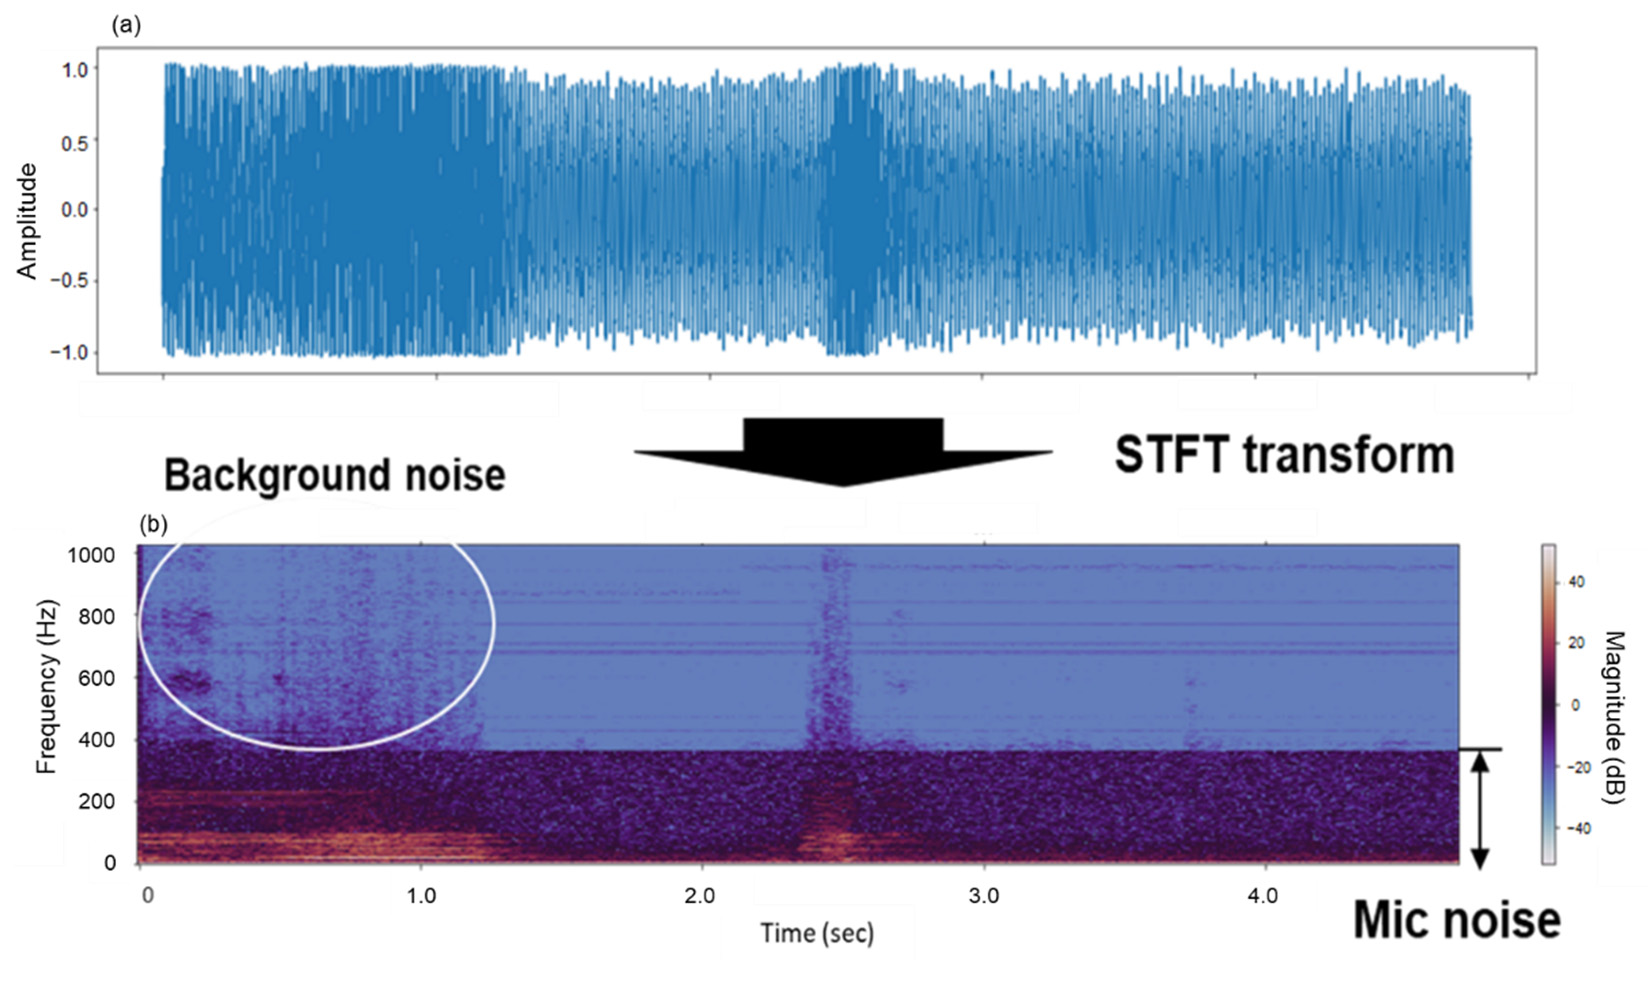
\includegraphics[width=0.8\textwidth]{./img/conversion}
    \caption{\label{fig:conversion}Tweedimensionale bron van de spraakgegevens van de oestrusoproep bij runderen (a) en de omzetting naar korte-tijd Fourier transform (STFT) gebied (b)~\autocite{Jung2021}.}
\end{figure}

\begin{figure}
    \centering
    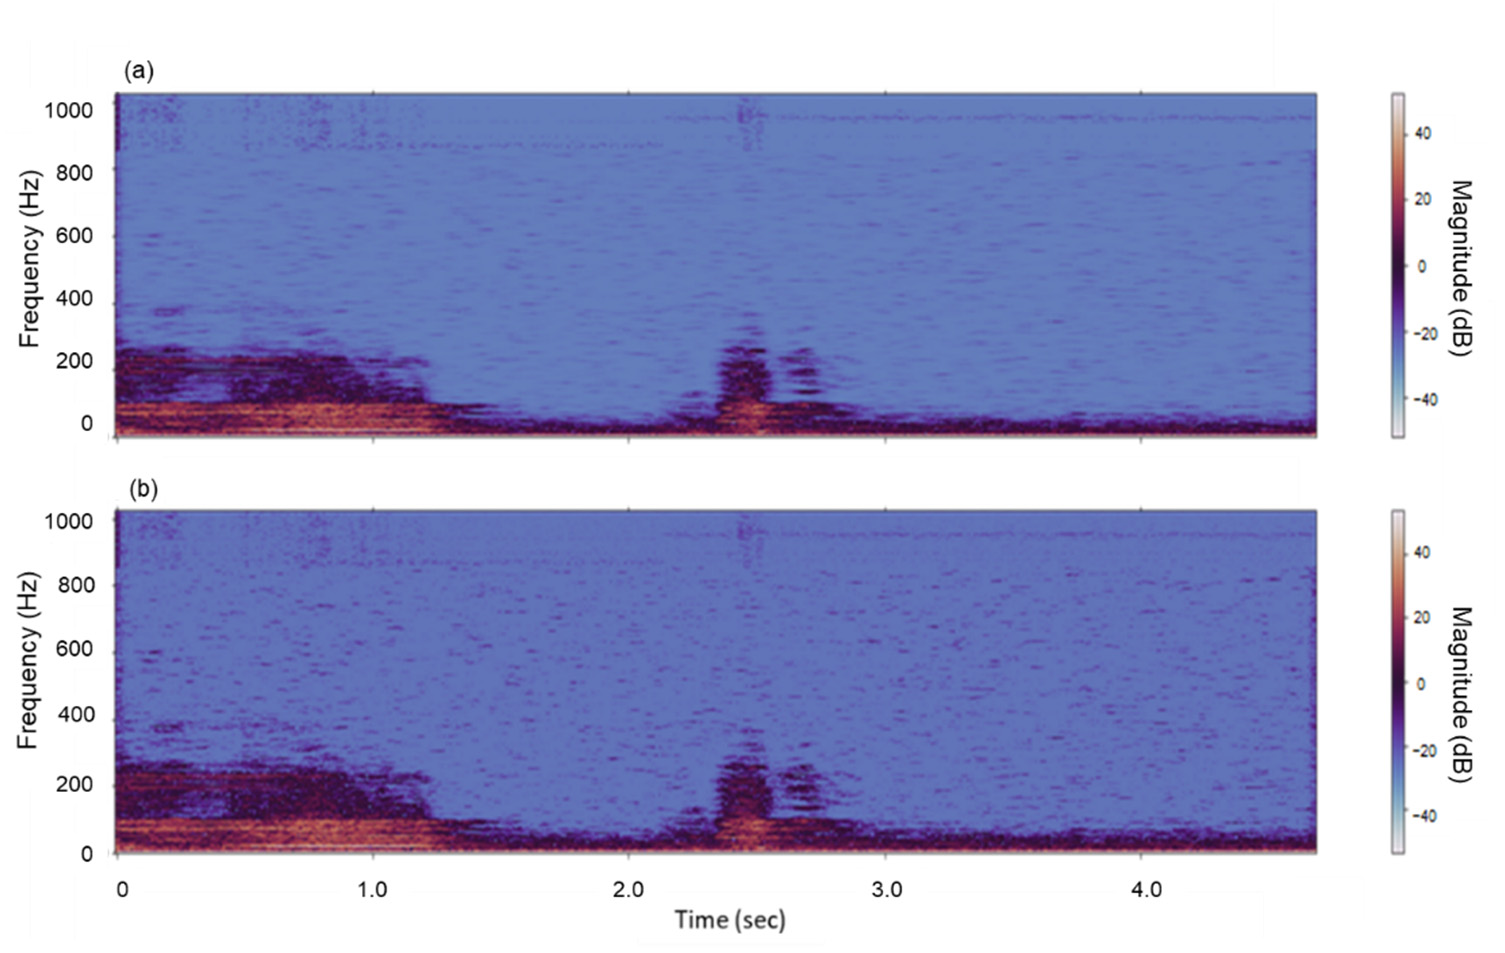
\includegraphics[width=0.8\textwidth]{./img/The_original_noise-removed_audio}
    \caption{\label{fig:The_original_noise-removed_audio}De originele audio met ruisonderdrukking (a) en spraakinformatie gecorrigeerd door ruismasker afvlakking (b)~\autocite{Jung2021}.}
\end{figure}

In de opstelling van het onderzoek van \textcite{Jung2021} gebruikt men de \textit{librosa} en de \textit{noisereduce} Python-bibliotheken. Deze twee bibliotheken zullen ook gebruikt worden in het praktische gedeelte van deze bachelorproef.
